\documentclass[10pt]{beamer}

\usetheme[progressbar=frametitle]{metropolis}
\usepackage{appendixnumberbeamer}

\usepackage{booktabs}
\usepackage[scale=2]{ccicons}


\usepackage{pgfplots}
\usepgfplotslibrary{dateplot}

\usepackage{xspace}
\newcommand{\themename}{\textbf{\textsc{metropolis}}\xspace}

\title{\LaTeX}
\subtitle{A Hands-On Session}
%\date{\today}
\date{Nov 7, 2019}
%\author{Matthias Vogelgesang}
%\institute{Center for modern beamer themes}
% \titlegraphic{\hfill\includegraphics[height=1.5cm]{logo.pdf}}

\begin{document}

\maketitle

\begin{frame}[fragile]{Hello World!}
\centering
\begin{figure}

\includegraphics[scale=0.5]{images/hello.png}
\caption{This will be today's first LaTeX output}
\end{figure}
\end{frame}

\begin{frame}[fragile]{Hello World!}
Our first document

\begin{verbatim}    
   \documentclass{article}
    
    \begin{document}
    Hello World
    \end{document}
\end{verbatim}

Using any text editor of your choice, save the above lines in a file named $'sample.tex'.$
%\end{frame}

%\begin{frame}[fragile]{Compilation from terminal}
% Some commands \vskip 0.5cm
% \begin{verbatim}
% latex sample.tex  
% \end{verbatim}
% The above command will output a .dvi file 
\pause \vskip 1cm
\begin{verbatim}
pdflatex sample.tex  
\end{verbatim}
The above command will output a .pdf file 
% \vskip 1.25cm
% \begin{verbatim}
% dvipdfm sample.dvi 
% \end{verbatim}
% The above command will convert \textit{sample.dvi} to a pdf file named \textit{sample.pdf}
\end{frame}

\begin{frame}[fragile]{Hands-on}
Create a folder 'handson1' \vskip 0.25cm

Create your own 'Hello World!' Latex document and compile it.

\end{frame}

\begin{frame}[fragile]{Document Class}
First line of the \textit{Hello World!} LaTeX program:
\begin{verbatim}
    \documentclass{article}
\end{verbatim} \pause
Base LaTeX offers four types of document classes.
  \begin{verbatim}   
  book
  report
  article
  letter
  \end{verbatim}

For each class, LaTeX provides a class file which can be loaded via the $documentclass$ command at the top of the document.
\end{frame}

\begin{frame}[fragile]{Let's give it a title!}
\centering
\begin{figure}
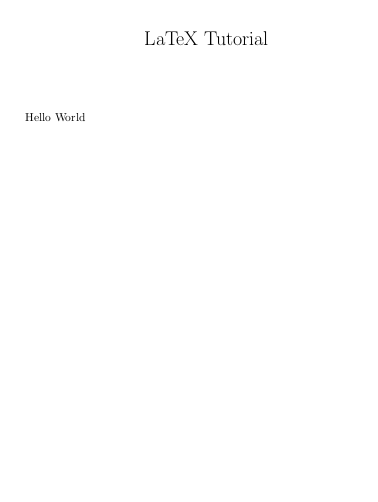
\includegraphics[scale=0.4]{images/title.png}
\end{figure}
\end{frame}

\begin{frame}[fragile]{Let's give it a title!}
\begin{verbatim}
    \documentclass{article}
    \title{LaTeX Tutorial}
    
\end{verbatim} \pause
\begin{verbatim}
    \begin{document}
        \maketitle  
        Hello World
    \end{document}
\end{verbatim}
\end{frame}


\begin{frame}[fragile]{Some more information...}
\begin{verbatim}
    \documentclass{article}
    \title{LaTeX Tutorial}
    \author{Devi}
    \date{\today}
\end{verbatim} \pause
\begin{verbatim}
    \begin{document}
        \maketitle  
        Hello World
    \end{document}
\end{verbatim}
\end{frame}

\begin{frame}[fragile]{Hands-on 2}
Create a new folder 'handson2' \vskip 0.25cm

Create a LaTeX document using the 'report' document class; add title, author names and date. \vskip 0.25cm

Do you see a difference between 'report' and 'article' document classes?
\end{frame}


\begin{frame}[fragile]{Let's add content to our document}
\begin{figure}
    \centering
    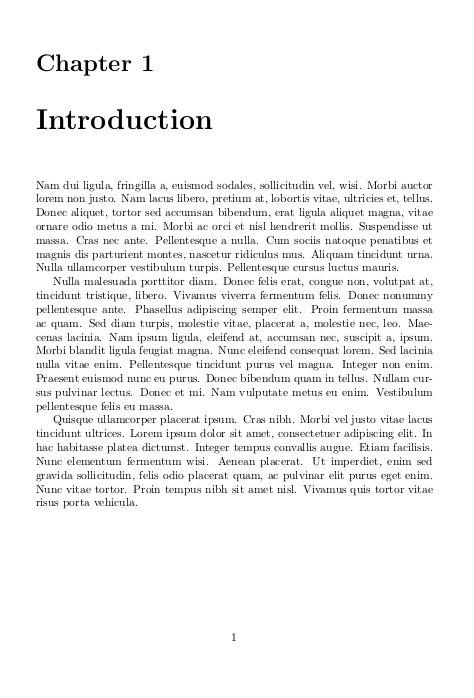
\includegraphics[scale=0.2]{images/chapter1.png}
    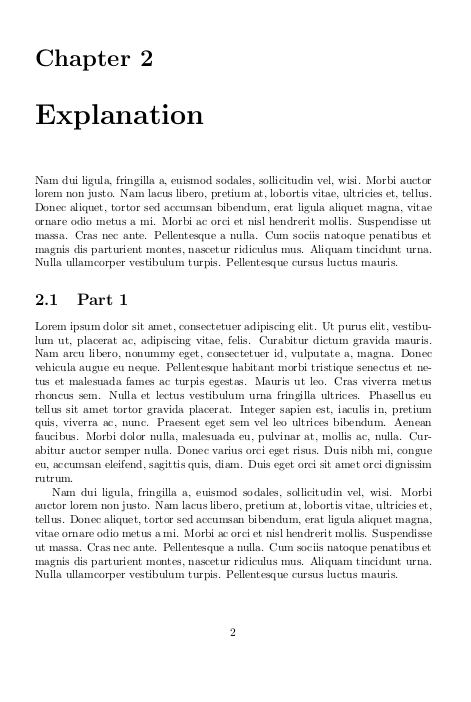
\includegraphics[scale=0.2]{images/chapter2.png}
    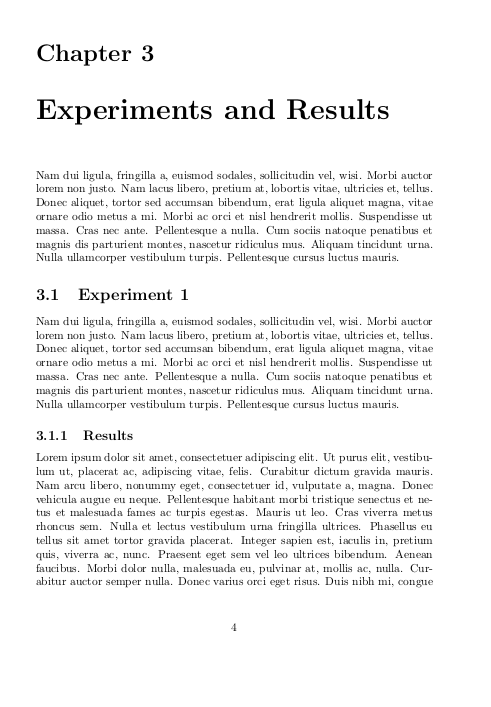
\includegraphics[scale=0.2]{images/chapter3.png}
\end{figure}
\end{frame}

\begin{frame}[fragile]{Let's add content to our document}
\small{\begin{verbatim}
\documentclass{report}
\title{LaTeX Tutorial}
\begin{document}
    \maketitle
    \chapter{Introduction}
    This chapter introduces the report content.\end{verbatim}\pause \begin{verbatim}
    \chapter{Explanation}
    This chapter explains the idea in detail
        \section{Part 1}
        Some content here.\end{verbatim}\pause\begin{verbatim}
    \chapter{Experiments and Results}
    This chapter discusses the experiments and results.
        \section{Experiment 1}
        Details about the first experiment goes here.
            \subsection{Results}
    \chapter{Conclusion}This chapter concludes the report.
\end{document}
\end{verbatim}
}
\end{frame}

\begin{frame}[fragile]{Hands-on 3}
Create a folder 'handson3' and copy the earlier documents to it. \vskip 0.25cm

Add chapters, sections and subsections to your report document.
\end{frame}

\begin{frame}[fragile]{Can we keep the document modular?}
From 
\begin{verbatim}
    sample.tex
\end{verbatim}
To
\begin{verbatim}
    main.tex
    introduction.tex
    chapter1.tex
    chapter2.tex
    conclusion.tex
\end{verbatim}
\end{frame}

\begin{frame}[fragile]{Can we keep the document modular?}
\small{
\textit{Contents of the file 'main.tex'}
\begin{verbatim}
    \documentclass{report}
    \title{LaTeX Tutorial}
    \begin{document}
        \maketitle
        \input{introduction}
        \input{chapter1}
        \input{chapter2}
        \input{conclusion}
    \end{document}
\end{verbatim}  \pause
\textit{Contents of the file 'introduction.tex'}
\begin{verbatim}
    \chapter{Introduction}
    This chapter introduces the report content.
\end{verbatim} }\pause 
Similarly, create \textit{chapter1.tex, chapter2.tex} and \textit{conclusion.tex}. \\
No separate preamble or \verb|\begin{document}| in these files.
\end{frame}

\begin{frame}[fragile]{Hands-on 4}
Create a folder 'handson4' and copy the earlier documents to it. \vskip 0.25cm

Make your report modular.
\end{frame}

\begin{frame}[fragile]{Part 1}

\begin{itemize}
    \item Typography, Fonts
    \item Ordered, Unordered Lists
    \item Images
    \item Tables
    \item Labels and References
\end{itemize}
\end{frame}

\begin{frame}[fragile]{Typography}
\begin{verbatim}
\textbf{boldface text}
\end{verbatim}

\begin{center}becomes\end{center}
\textbf{boldface text}
\end{frame}

\begin{frame}[fragile]{Some font options...}

\begin{tabular}{ll}
Font Style  &  LaTeX command \\
\hline \\
\emph{Emphasize} & \verb|\emph{Emphasize}| \\ \pause
\textit{Italic} & \verb|\textit{Italic}| \\
\textsc{SmallCaps} & \verb|\textsc{SmallCaps}| \\
\textbf{Bold} & \verb|\textbf{Bold}| \\
\textbf{\textit{Bold Italic}} & \verb|\textbf{\textit{Bold Italic}}| \\
\textbf{\textsc{Bold SmallCaps}} & \verb|\textbf{\textsc{Bold SmallCaps}}| \\ \pause
\footnotesize{Footnote Size} & \verb|\footnotesize{Footnote Size}| \\
{\small Small} & \verb|{\small Small}| \\
{\large large} & \verb|{\large large}| \\
{\Large Large} & \verb|{\Large Large}| \\
{\LARGE LARGE} & \verb|{\LARGE LARGE}| \\
{\huge huge} & \verb|{\huge huge}| \\
{\Huge Huge} & \verb|{\Huge Huge}| \\
\end{tabular}
\end{frame}


\begin{frame}[fragile]{Hands-on 5}
Create a folder 'handson5' and copy the earlier documents to it. \vskip 0.25cm

Play with the font options.
\end{frame}

\begin{frame}[fragile]{Lists}
  \begin{columns}[T,onlytextwidth]
    \column{0.25\textwidth}
      Items
      \begin{itemize}
        \item Milk \item Eggs \item Potatos
      \end{itemize} \pause

    \column{0.25\textwidth}
      Enumerations
      \begin{enumerate}
        \item First, \item Second, \item Last.
      \end{enumerate} \pause

    \column{0.5\textwidth}
      Descriptions
      \begin{description}
        \item[Table] A type of furniture. \item[Plate] A type of utensil.
        \item[Pencil] A stationary item.
      \end{description}
  \end{columns}
\end{frame}

\begin{frame}[fragile]{Unordered list using the environment Itemize}
  \begin{columns}[T,onlytextwidth]
    \column{0.4\textwidth}
     Unordered List
      \begin{itemize}
        \item Milk 
        \item Eggs 
        \item Potatos
      \end{itemize}

    \column{0.5\textwidth}
     \begin{verbatim}
      \begin{itemize}
        \item Milk 
        \item Eggs 
        \item Potatos
      \end{itemize}
    \end{verbatim} 
   \end{columns}  
   
\end{frame}

\begin{frame}[fragile]{Ordered List using the environment  Enumerate}
  \begin{columns}[T,onlytextwidth]
    \column{0.4\textwidth}
     Ordered List
      \begin{enumerate}
        \item First, 
        \item Second,
        \item Last.
      \end{enumerate}
    
    \column{0.5\textwidth}
      Ordered List 
      \begin{verbatim}
      \begin{enumerate}
        \item First, 
        \item Second,
        \item Last.
      \end{enumerate}
    \end{verbatim}
   \end{columns}  
\end{frame}

\begin{frame}[fragile]{A list of descriptions using the environment Description}
  
      Descriptions
      \begin{description}
        \item[Table] A type of furniture.
        \item[Plate] A type of utensil.
        \item[Pencil] A stationary item.
      \end{description}

\begin{verbatim}
\begin{description}
    \item[Table] A type of furniture.
    \item[Plate] A type of utensil.
    \item[Pencil] A stationary item.
\end{description}
\end{verbatim}
\end{frame}

\begin{frame}[fragile]{Hands-on 6}

Create a folder 'handson6' and copy the earlier documents to it. \vskip 0.25cm

List down three of your favourite food items using \verb|itemize, enumerate| and \verb|description|.

\end{frame}

\begin{frame}[fragile]{Figures}
  \begin{figure}
    \includegraphics[width=0.5\textwidth]{./images/knuth.jpg}
    \caption{Donald Knuth, creator of TeX}
  \end{figure}
\end{frame}

\begin{frame}[fragile]{Figures}
 \begin{verbatim}
\begin{figure}
    \includegraphics[width=0.5\textwidth]{./knuth.jpg}
    \caption{Donald Knuth, creator of TeX}
\end{figure}
 \end{verbatim}
\end{frame}

\begin{frame}[fragile]{Labels and References}
\begin{verbatim}
\begin{figure}
    \includegraphics[width=0.5\textwidth]{./knuth.jpg}
    \caption{Donald Knuth, creator of TeX}
    \label{fig:knuth}
\end{figure}
\end{verbatim}
\verb|\label| should always come after \verb|\caption|. \\ \pause
\verb|\label{knuth}| is also a valid label... 'fig:' is used as a good naming convention. \\~\\ \pause 

{\color{blue}\textbf{How to refer to a figure by its label?}}\\ \pause
Figure \verb|\ref{fig:knuth}| is that of Donald Knuth. \pause
\begin{center}becomes \end{center}
Figure 1 is that of Donald Knuth.
\end{frame}

\begin{frame}[fragile]{Hands-on 7}

Create a folder 'handson7' and copy the earlier documents to it. \vskip 0.25cm

Include your image in the LaTeX document using the \verb|figure| environment. \vskip 0.25cm

Give your figure a fitting caption using \verb|\caption|. \vskip 0.25cm

Label your figure using \verb|\label|. \vskip 0.25cm

Refer to your image by its label using \verb|\ref| and write few lines about it.

\end{frame}


\begin{frame}[fragile]{Tables}
  \begin{table}
    \caption{Largest cities in the world (source: Wikipedia)}
    \begin{tabular}{lr}
      \hline
      City & Population\\
      \hline
      Mexico City & 20,116,842\\
      Shanghai & 19,210,000\\
      Peking & 15,796,450\\
      Istanbul & 14,160,467\\
      \hline
    \end{tabular}
  \end{table}
\end{frame}


\begin{frame}[fragile]{Tables}
\begin{verbatim}
\begin{table}
\caption{Largest cities in the world (src: Wikipedia)}
    \begin{tabular}{ll}
        \hline
        City        &   Population\\
        \hline
        
        Mexico City &   20,116,842\\
        Shanghai    &   19,210,000\\
        Peking      &   15,796,450\\
        Istanbul    &   14,160,467\\
        \hline
    \end{tabular}
\end{table}
\end{verbatim}
\end{frame}



\begin{frame}[fragile]{Labels and References}
\begin{verbatim}
\begin{table}
    \begin{tabular}{cc}
        ... & ... 
    \end{tabular}
    \caption{A dummy table}
    \label{tab:dummy}
\end{table}
\end{verbatim}
\verb|\label| should always come after \verb|\caption|. \\ \pause
\verb|\label{dummy}| is also a valid label... 'tab:' is used as a good naming convention. \\~\\ \pause 

{\color{blue}\textbf{How to refer to a table by its label?}}\\ \pause
Table \verb|\ref{tab:dummy}| is  a dummy table. 
\end{frame}


\begin{frame}[fragile]{Labels and References}

{\color{blue}\textbf{How to label a section?}}\\ \pause
\begin{verbatim}
\section{Introduction \label{sec:intro}}
\end{verbatim}

{\color{blue}\textbf{Referring to a section..}}\\~\\ \pause
Section \verb|\ref{sec:intro}| introduces the proposed method. 
\end{frame}

\begin{frame}[fragile]{Hands-on 8}

Create a folder 'handson8' and copy the earlier documents to it. \vskip 0.25cm


Tabulate the roll numbers and names of 5 students using the \verb|table| environment. \vskip 0.25cm

Give your table a fitting caption using \verb|\caption|. \vskip 0.25cm

Label your table using \verb|\label|. \vskip 0.25cm

Refer to your table by its label using \verb|\ref| and write few lines about it.

\end{frame}


\begin{frame}[fragile]{Part 2}

\begin{itemize}
    \item Math
    \item Packages
    \item Citations and Bibliography
\end{itemize}
\end{frame}

\begin{frame}[fragile]{Math}

\textit{Inline Math Usage} \vskip 0.5cm
"This report discusses the function $y=x$ and its properties." \pause

\begin{verbatim}
This report discusses the function $ y=x $ and 
its properties
\end{verbatim}  

\verb|$..$| marks the beginning and end of the inline math environment.

\end{frame}

\begin{frame}[fragile]{Math}

\textit{Inline Math Usage} \vskip 0.5cm
"The next function to be discussed is $ y=x^2 $." \pause

\begin{verbatim}
The next function to be discussed is $ y=x^2 $.
\end{verbatim} 

\end{frame}

\begin{frame}[fragile]{Math}

\textit{Math Equation} \vskip 0.5cm
This report discusses the below equation.
\begin{equation}
    y= x^2
\end{equation} \pause

\begin{verbatim}
This report discusses the below equation.
\begin{equation}
    y= x^2
\end{equation}
\end{verbatim}  \pause

\end{frame}

\begin{frame}[fragile]{Math}

\textit{Math Equation} \vskip 0.5cm
This report discusses the below equation.
\begin{equation*}
    y= x^2
\end{equation*} \pause

\begin{verbatim}
This report discusses the below equation.
\begin{equation*}
    y= x^2
\end{equation*}
\end{verbatim}  \pause

\verb|equation*| suppresses the numbering.
\end{frame}

\begin{frame}[fragile]{Math}

\textit{Math Equation} \vskip 0.5cm
Equation \ref{eq:frac} demonstrates how to write fractions in LaTeX.

\begin{equation}
    y= \frac{1}{x}
    \label{eq:frac}
\end{equation} \pause

\small{
\begin{verbatim}
Equation \ref{eq:xsquare} demonstrates how to write fractions in LaTeX.

\begin{equation}
    y= \frac{1}{x}
    \label{eq:frac}
\end{equation} 
\end{verbatim}}

\end{frame}



\begin{frame}[fragile]{Math}
An example to inspire the use of LaTeX for mathematical writing.
\begin{equation*}
  \mbox{Value of }  e = \lim_{n\to \infty} \left(1 + \frac{1}{n}\right)^n
\end{equation*} \pause
\small{
\begin{verbatim}
\begin{equation}
    \mbox{Value of} e = \lim_{n \to \infty} \left(1
                        + \frac{1}{n} \right)^n
\end{equation}
\end{verbatim}}  \pause
  
\begin{tabular}{ll}
Symbol  & LaTeX command \\
\toprule
Text inside equations  & \verb|\mbox| \\
$\to$ & \verb|\to|\\
$\infty$ & \verb|\infty| \\
$\left($ & \verb|\left(| \\
$\frac{1}{n}$ & \verb|\frac{1}{n}| \\
$x^n$  & \verb|x^n|
\end{tabular}

\end{frame}

\begin{frame}[fragile]{Math}

Equation array using \verb|eqnarray|. 
No need to include any packages. Comes with base LaTeX. 

\begin{eqnarray}
(x+y)^3&=& (x+y)(x+y)^2\\
       &=& (x+y)(x^2+2xy+y^2)\\
       &=& x^3+3x^2y+3xy^3+x^3.
\end{eqnarray} \pause

\begin{verbatim}
\begin{eqnarray}
    (x+y)^3 &=& (x+y)(x+y)^2        \\
            &=& (x+y)(x^2+2xy+y^2)  \\
            &=& x^3+3x^2y+3xy^3+x^3.
\end{eqnarray}
\end{verbatim}

\end{frame}

\begin{frame}[fragile]{Math}

Equation array using \verb|align|. 
Must include \verb|\usepackage{amsmath}|.

\begin{align}
(x+y)^3&=(x+y)(x+y)^2\\
      &=(x+y)(x^2+2xy+y^2)\\
      &=x^3+3x^2y+3xy^3+x^3.
\end{align} \pause

\begin{verbatim}
\begin{align}
    (x+y)^3 &= (x+y)(x+y)^2        \\
            &= (x+y)(x^2+2xy+y^2)  \\
            &= x^3+3x^2y+3xy^3+x^3.
\end{align}
\end{verbatim}

\end{frame}

\begin{frame}[fragile]{Hands-on 9}

Create a folder 'handson9' and copy the earlier documents to it. \vskip 0.25cm

Try the following: \vskip 0.25cm
\small{
Let $a$ and $b$ be two variables. 
Then $(a+b)^2$ can be calculated as follows:
\begin{eqnarray}
(a+b)^2 &=& (a+b)(a+b) \\
        &=& a^2 + ab + ba + b^2 \\
        &=& a^2 + 2ab + b^2
\end{eqnarray}}

\begin{verbatim}
Let $a$ and $b$ be two variables. Then $(a+b)^2$ can be 
calculated as follows:

\begin{eqnarray}
(a+b)^2 &=& (a+b)(a+b) \\
        &=& a^2 + ab + ba + b^2 \\
        &=& a^2 + 2ab + b^2
\end{eqnarray}
\end{verbatim}
\end{frame}

%%%%%%%%%%%%%%%%% part2%%%%%%%%%%%%%%%
\begin{frame}[fragile]{Packages}

\url{https://www.ctan.org/pkg/} \vskip 0.5cm

\textbf{Some packages...}\\
graphicx \\
amsmath \\
amsfonts \\
hyperref \\
beamer \\
tikz\\
geometry \\
xcolor \\
pgfplots \\
subfigure \\
natbib 
\end{frame}

\begin{frame}[fragile]{Package amsmath}
\verb|\usepackage{amsmath}|
$$
\begin{matrix}
a & b \\
c & d
\end{matrix}
\quad
\begin{pmatrix}
a & b \\
c & d
\end{pmatrix}
\quad
\begin{bmatrix}
a & b \\
c & d
\end{bmatrix}
\quad
\begin{vmatrix}
a & b \\
c & d
\end{vmatrix}
\quad
\begin{Vmatrix}
a & b \\
c & d
\end{Vmatrix}
$$

\end{frame}

\begin{frame}[fragile]{Package amsmath}

\verb|\usepackage{amsmath}|

\begin{columns}
\column{0.45\textwidth}
\begin{verbatim}
\begin{matrix}
a & b \\
c & d
\end{matrix} 
\end{verbatim} 
\column{0.45\textwidth}
\begin{matrix}
a & b \\
c & d
\end{matrix} \\
\end{columns}

\begin{columns}
\column{0.45\textwidth}
\begin{verbatim}
\begin{pmatrix}
a & b \\
c & d
\end{pmatrix} 
\end{verbatim} 
\column{0.45\textwidth}
\begin{pmatrix}
a & b \\
c & d
\end{pmatrix} \\
\end{columns}

\begin{columns}
\column{0.45\textwidth}
\begin{verbatim}
\begin{bmatrix}
a & b \\
c & d
\end{bmatrix} 
\end{verbatim} 
\column{0.45\textwidth}
\begin{bmatrix}
a & b \\
c & d
\end{bmatrix} \\
\end{columns}
\end{frame}

\begin{frame}[fragile]{Package amsmath}

\verb|\usepackage{amsmath}|
\begin{columns}
\column{0.45\textwidth}
\begin{verbatim}
\begin{vmatrix}
a & b \\
c & d
\end{vmatrix} 
\end{verbatim} 
\column{0.45\textwidth}
\begin{vmatrix}
a & b \\
c & d
\end{vmatrix} \\
\end{columns}

\begin{columns}
\column{0.45\textwidth}
\begin{verbatim}
\begin{Vmatrix}
a & b \\
c & d
\end{Vmatrix} 
\end{verbatim} 
\column{0.45\textwidth}
\begin{Vmatrix}
a & b \\
c & d
\end{Vmatrix} \\
\end{columns}
\end{frame}

\begin{frame}[fragile]{Package Tikz}
To get started with TikZ we need to load up the tikz package:

\verb|\usepackage{tikz}| \pause 

Now whenever we want to create a TikZ diagram we need to use the tikzpicture environment.

\begin{verbatim}
\begin{tikzpicture}
    <code goes here>
\end{tikzpicture}
\end{verbatim} \pause

Nice tutorial for beginners here:\vskip 0.15cm
\footnotesize{\url{https://www.overleaf.com/learn/latex/LaTeX_Graphics_using_TikZ:_A_Tutorial_for_Beginners_(Part_1)%E2%80%94Basic_Drawing}}

\end{frame}



\begin{frame}[fragile]{Citations and Bibliography}
\begin{figure}
    \centering
    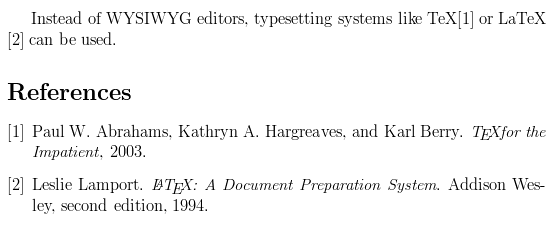
\includegraphics[scale =0.5]{images/bib.jpeg}
\end{figure}
\end{frame}

\begin{frame}[fragile]{Citations and Bibliography}
Get the \textit{bibTeX} entries for the references.
\begin{verbatim}
@book{golumbic2004algorithmic,
        title={Algorithmic graph theory and perfect graphs},
        author={Golumbic, Martin Charles},
        volume={57},
        year={2004},
        publisher={Elsevier}
}
\end{verbatim}
You can use  \textit{bibtex generators, google scholar, dblp, etc} to get the above file. \vskip 0.25cm
Create a \textit{.bib} file with the bibTeX entries.
\end{frame}

\begin{frame}[fragile]{Citations and Bibliography}

\begin{verbatim}
\documentclass{report}
\usepackage{biblatex}
\begin{document}
    \section{Introduction}
    A good introduction to graph algorithms can be
    found in \cite{golumbic2004algorithmic}. 
    ....
\end{verbatim} \pause \begin{verbatim} 
    \bibliographystyle{plain}
    \bibliography{ref}
\end{document}
\end{verbatim}
We assume that your bibliography file is \textit{ref.bib}. To Compile: \vskip 0.1cm
    \verb|pdflatex -> bibtex -> pdflatex -> pdflatex|

\end{frame}

\begin{frame}[fragile]{Hands-on 10}

Create a folder 'handson10' and copy the earlier documents to it. \vskip 0.25cm

Create a  .bib file with a single bibTeX entry \vskip 0.5cm

Cite it and write a few lines in the main LaTeX document.
\end{frame}

%%%%%%%%%%%%%%%%% part5%%%%%%%%%%%%%%%
\begin{frame}[fragile]{Online LaTeX Editors}

Overleaf
\end{frame}

\begin{frame}[fragile]{Standalone LaTeX Editors}
TeXmaker \vskip 0.5cm
TeXStudio \vskip 0.5cm
TeXShop \vskip 0.5cm
Lyx \vskip 0.5cm
TeXpen \vskip 0.5cm
Gummi \vskip 0.5cm
...

\end{frame}

%%%%%%%%%%%%%%%%% part6%%%%%%%%%%%%%%%
\begin{frame}[fragile]{Advanced}
Macros  - user defined short-hands for complex LaTeX formulas\vskip 0.5cm
Beamer - package to create LaTeX presentations \vskip 0.5cm
pgfplots - package for creating graphs, figures, etc \vskip 0.5cm
\end{frame}


\end{document}
